\documentclass{article}

\usepackage{amsmath, amsthm, amssymb, amsfonts}
\usepackage{thmtools}
\usepackage{graphicx}
\usepackage{setspace}
\usepackage{geometry}
\usepackage{float}
\usepackage{hyperref}
\usepackage[utf8]{inputenc}
\usepackage[english]{babel}
\usepackage{framed}
\usepackage[dvipsnames]{xcolor}
\usepackage{tcolorbox}

\colorlet{LightGray}{White!90!Periwinkle}
\colorlet{LightOrange}{Orange!15}
\colorlet{LightGreen}{Green!15}

\newcommand{\HRule}[1]{\rule{\linewidth}{#1}}

\declaretheoremstyle[name=Theorem,]{thmsty}
\declaretheorem[style=thmsty,numberwithin=section]{theorem}
\tcolorboxenvironment{theorem}{colback=LightGray}

\declaretheoremstyle[name=Proposition,]{prosty}
\declaretheorem[style=prosty,numberlike=theorem]{proposition}
\tcolorboxenvironment{proposition}{colback=LightOrange}

\declaretheoremstyle[name=Principle,]{prcpsty}
\declaretheorem[style=prcpsty,numberlike=theorem]{principle}
\tcolorboxenvironment{principle}{colback=LightGreen}

\theoremstyle{definition}
\newtheorem{definition}{Definition}[section]

\theoremstyle{remark}
\newtheorem*{remark}{Remark}

\newcommand{\argmin}{\mathop{\mathrm{argmin}}}
\newcommand{\argmax}{\mathop{\mathrm{argmax}}}
\newcommand{\minimize}{\mathop{\mathrm{minimize}}}
\newcommand{\maximize}{\mathop{\mathrm{maximize}}}
\newcommand{\st}{\mathop{\mathrm{subject\,\,to}}}
\newcommand{\tab}[1][1cm]{\hspace*{#1}}

\def\R{\mathbb{R}}
\def\E{\mathbb{E}}
\def\P{\mathbb{P}}
\def\S{\mathbb{S}}
\def\Cov{\mathrm{Cov}}
\def\Var{\mathrm{Var}}
\def\half{\frac{1}{2}}
\def\sign{\mathrm{sign}}
\def\supp{\mathrm{supp}}
\def\th{\mathrm{th}}
\def\tr{\mathrm{tr}}
\def\dim{\mathrm{dim}}
\def\dom{\mathrm{dom}}


\def\hwnum{3}


\setstretch{1.2}
\geometry{
    textheight=9in,
    textwidth=5.5in,
    top=1in,
    headheight=12pt,
    headsep=25pt,
    footskip=30pt
}

% ------------------------------------------------------------------------------

\begin{document}

% ------------------------------------------------------------------------------
% Cover Page and ToC
% ------------------------------------------------------------------------------

\title{ \normalsize \textsc{}
		\\ [2.0cm]
		\HRule{1.5pt} \\
		\LARGE \textbf{\uppercase{Gradient Descent}
		%\HRule{2.0pt} \\ [0.6cm] \LARGE{Subtitle}
        \vspace*{10\baselineskip}}
		}
\date{}
\author{\textbf{Author} \\ 
		Vinitra Muralikrishnan \\
		11th March, 2024}

\maketitle
\newpage

\tableofcontents
\newpage

% ------------------------------------------------------------------------------

\section{Overview}

\begin{definition}
    It is an algorithm for minimizing a differentiable function.
\end{definition}

\subsection{Update rule}
$x_k = x_{k-1} - t_k \nabla f(x_{k-1})$.
where, $t_k$ can be fixed or adaptive.\\

\subsection{Basic algorithm}
\begin{enumerate}
    \item{}choose initial point $x_0 \in \R$
    \item{}repeat $x_k = x_{k-1} - t_k \nabla f(x_{k-1})$
    \item{} stop for instnce when objective decreases by less than $\epsilon$ (user parameter).
\end{enumerate}

\subsection{Adaptive step size algorithm / Backtracking line search}
\begin{enumerate}
    \item{}Set $x_0,\ \alpha_{0} > 0,\ 0 < \rho < 1$
    \item{}On each iteration k:
    \item{}\tab $f_k \leftarrow f(x_k)$
    \item{}\tab Set $d_k \leftarrow -\nabla f(x_{k-1})$
    \item{}\tab $\alpha \leftarrow \alpha_0$
    \item{}\tab while $f(x_k + \alpha d_k) \geq f_k: \alpha \leftarrow \rho \alpha$
    \item{}\tab $x_{k+1} \leftarrow x_k + \alpha d_k$
\end{enumerate}

\subsubsection{Exact line search}
Can we choose the ideal step direction?\\
This would also be a minimization problem as follows:
$$t = \argmin_{s \geq 0} f(x - s\nabla f(x))$$
\textbf{Answer: } No
\begin{itemize}
    \item approximation is not as efficient as backtracking
    \item not worth solving yet another minimization problem for an existing one
\end{itemize}

\section{Convergence Analysis}

\section{Considerations}
\subsection{Pros and Cons}
\textbf{Pros}
\begin{itemize}
    \item simple idea
    \item low computational cost per iterations
    \item fast for problems that are well-conditioned and strongly convex
\end{itemize}
\textbf{Cons}
\begin{itemize}
    \item Slow for problems not strongly convex
    \item slow if problem not well conditioned
    \item only applicable to differentiable functions
\end{itemize}
%\begin{theorem}
    %This is a theorem.
%\end{theorem}

%\begin{proposition}
    %This is a proposition.
%\end{proposition}

%\begin{principle}
    %This is a principle.
%\end{principle}

%% Maybe I need to add one more part: Examples.
%% Set style and colour later.

%\subsection{Pictures}

%\begin{figure}[htbp]
    %\center
    %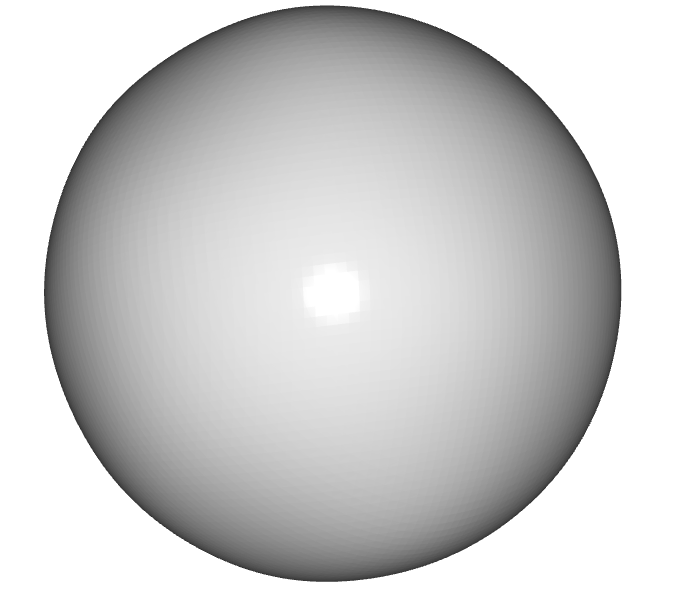
\includegraphics[scale=0.06]{img/photo.png}
    %\caption{Sydney, NSW}
%\end{figure}

%\subsection{Citation}

%This is a citation\cite{Eg}.

%\newpage

% ------------------------------------------------------------------------------
% Reference and Cited Works
% ------------------------------------------------------------------------------

\bibliographystyle{IEEEtran}
\bibliography{References.bib}

% ------------------------------------------------------------------------------

\end{document}
